% +--------------------------------------------------------------------+
% | Sample Chapter 3
% +--------------------------------------------------------------------+

\cleardoublepage

% +--------------------------------------------------------------------+
% | Replace "This is Chapter 3" below with the title of your chapter.
% | LaTeX will automatically number the chapters.
% +--------------------------------------------------------------------+

\chapter{Exploración Hardware}
\label{makereference3}

\section{Objetivos de la exploración: descubrir variedad de dispositivos y especificaciones}
\label{makereference3.1}

El objetivo inicial del proyecto a nivel técnico era encontrar una placa de desarrollo que incluyera Bluetooth de bajo consumo y permitiera conectar  un sensor de acelerometría, ya que eran indispensables para la transmisión de datos entre la placa y el dispositivo móvil. 

Desde el punto de vista comercial, la intención ha sido buscar el componente con mejores prestaciones en calidad y precio con el objetivo de preparar un producto final que pudiera competir con otras opciones del mercado.

Destacamos dos grupos: placas con bluetooth incorporado y componentes sólo con  bluetooth. En las tablas~\ref{tablaSoCBLE} y~\ref{tablaBLE} observamos el análisis de cada grupo.

\begin{table}
	\begin{center}
	\begin{tabular}[c]{|c|c|c|c|c|c|c|}
        \hline
        \multicolumn{7}{r}{CHIPS CON BLUETOOTH} \\
        \hline
        EMPRESA & MODELO & PRECIO(EUROS) & PROCESADOR & MEMORIA FLASH & MEMORIA RAM & I/O \\
        \hline
        Nordic & PTR9022 & 5,99 & ARM Cortex-M0 32 bit & 256 KB & 16 KB & SPI, 2-WIRE, UART \\
        Nordic & PTR9022 & 5,99 & ARM Cortex-M0 32 bit & 256 KB & 16 KB & SPI, 2-WIRE, UART \\
    	\hline
	\end{tabular}
    \caption{Placas que integran radio Bluetooth Low Energy. En verde, las alternativas seleccionadas para la siguiente fase de exploración}
    \label{tablaSoCBLE}
   \end{center}
\end{table}

\begin{table}
	\begin{center}
	\begin{tabular}[c]{|c|c|c|c|c|c|c|}
        \hline
        \multicolumn{7}{r}{CHIPS CON BLUETOOTH} \\
        \hline
        EMPRESA & MODELO & PRECIO(EUROS) & PROCESADOR & MEMORIA FLASH & MEMORIA RAM & I/O \\
        \hline
        Nordic & PTR9022 & 5,99 & ARM Cortex-M0 32 bit & 256 KB & 16 KB & SPI, 2-WIRE, UART \\
        Nordic & PTR9022 & 5,99 & ARM Cortex-M0 32 bit & 256 KB & 16 KB & SPI, 2-WIRE, UART \\
    	\hline
	\end{tabular}
    \caption{Chips solo BLE}
    \label{tablaBLE}
   \end{center}
\end{table}

\section{Plataformas cosideradas}
\label{makereference3.2}

Las empresas consideradas para comprar la placa de desarrollo con microprocesador fueron Nordic, Texas Instruments (TI) y Cypress.

En el grupo analizado para chips con Bluetooth sin procesador contemplamos las empresas Nordic,  Texas Instruments (TI), CSR y Dialog. 

Al considerar que era más interesante tener una placa con procesador, sensores y periféricos descartamos los chips individuales y optamos por una opción más completa.

\section{Criterios para la selección}
\label{makereference3.3}

\subsection{Aspectos técnicos}
\label{makereference3.3.1}

Realizado el primer filtro destacamos las que aparecen en la tabla~\ref{tablaSoCBLE}, podemos resaltar varias características importantes que tuvimos en cuenta.

El \textbf{procesador} es una característica fundamental, es el circuito integrado central más complejo encargado de interpretar y ejecutar instrucciones y de procesar datos con un mínimo consumo de energía. 
Como podemos observar en la tabla de microprocesadores con bluetooth predomina el núcleo \textbf{ARM Cortex-M0} de bajo consumo.

\textbf{ARM} Es el acrónimo de Advanced RISC Machines (ARM), una empresa conjunta entre Acorn Computers, Apple Computer (ahora Apple Inc.) y VLSI Technology.

Son microprocesadores RISC, acrónimo de Reduced Instruction Set Computing, computación de instrucciones reducidas. Esto quiere decir que se necesitan cargar  las instrucciones  de los datos de memoria a un registro antes de trabajar con ellos. Permite con esta tecnología reducir el consumo de energía con el mismo rendimiento computacional.

Estos procesadores soportan la arquitectura Thumb, que se emplea en algunos procesadores ARM para aplicaciones que necesiten mejorar la densidad de código. Consiste en usar un conjunto de instrucciones de 16 bits que es una forma comprimida del set de instrucciones ARM de 32 bits.
Observamos que la mayoría de los procesadores eran ARM Cortex-M0 32 bit.

Otro aspecto a considerar es la \textbf{memoria flash}, esta permite tanto la creación rápida de prototipos y la programación en el sistema. Es un tipo de memoria electrónica no volátil que se puede borrar y reprogramar fácilmente.
En estos microprocesadores se utiliza también para mantener códigos de control, por ejemplo los comandos básicos para manejos de dispositivos de entrada y salida del sistema (BIOS).
En nuestra búsqueda vimos que había de dos capacidades, de 256 KB y 128KB, con la opción de menor capacidad cubría las necesidades del proyecto.

La memoria RAM es importante,ya que gestiona la capacidad de datos que puede manejar el procesador. Es una memoria volátil, es decir que almacena los datos de forma temporal y al apagar la placa de la fuente de alimentación, se pierde su contenido.
En la búsqueda pudimos encontrar de dos tipos de almacenamiento tanto de  256 KB como de 128 KB.

En cuanto a los periféricos de entrada-salida, necesitábamos que la placa tuviera un protocolo de envío de datos maestro-esclavo, la mayoría de las placas de desarrollo incluyen protocolos SPI e I2C.

El protocolo \textbf{SPI} consiste en el envío de la señal de reloj del maestro y en cada impulso de reloj se envía un bit al esclavo y recibe un bit de éste. Los nombres de las señales son SCK para el reloj, MOSI para el Maestro Out Esclavo In, y MISO para Maestro In Esclavo Out.

El protocolo \textbf{I2C} es síncrono, usa dos cables, uno para el reloj (SCL) y otro para el dato (SDA). El maestro y esclavo envían datos por el mismo cable, el cual es controlado por el maestro, que crea la señal de reloj. Este protocolo utiliza direccionamiento, es decir, el primer byte enviado por el maestro se forma de 7 bits para la dirección (así que permite comunicarse con hasta 127 dispositivos) y un bit de lectura/escritura, indicando si el próximo byte vendrá desde el maestro o el esclavo.

Tras cada byte recibido se envía una confirmación con el noveno pulso de reloj. Si el maestro quiere recibir datos sólo genera pulsos de reloj. El esclavo tiene que cuidar que el próximo bit esté listo cuando la señal de reloj es dada. Dos o más señales a través del mismo cable pueden causar conflicto, y habría problemas si un dispositivo envía un 1 lógico al mismo tiempo que otro envía un 0. Por tanto el bus es "cableado" con resistencias de pull-up para poner el bus a nivel alto, y son los dispositivos los que fuerzan niveles bajos para enviar un ‘0’ lógico. Si quieren enviar un nivel alto simplemente lo comunican al bus.

\subsection{Aspectos calidad-precio}
\label{makereference3.3.2}

Destacar primeramente el proveedor, debe ser una empresa consolidada y especializada del sector de componentes electrónicos, que ofrezcan productos competentes y de calidad y que la respalde un buen soporte y una gran comunidad para posibles dudas técnicas.

El precio es fundamental que no se exceda, ya que el producto final podría encarecerse y no ser competente ni atractivo de cara al público objetivo.

En nuestro caso valoramos como opción inicial realizar las pruebas del proyecto sobre una placa desarrollo que incluye un kit completo con múltiples componentes, rondando los 50 euros. 

Por lo tanto es un paso intermedio entre las pruebas iniciales con la placa y lo que sería el procesador ya preparado y cableado antes de llevarlo incorporado como producto final.

\section{Plataformas escogidas}
\label{makereference3.4}

Rápidamente observamos dos grandes empresas especializadas en el sector como son Nordic y Cypress. Tienen gran variedad de microprocesadores y placas de desarrollo que cumplen con nuestras expectativas.

Aunque el precio es más elevado, nos decantamos por el kit de desarrollo de Nordic (\textbf{nRF51-DK}) este que incluye Bluetooth Smart, y protocolo de operación  ANT a 2.4GHz. Incorpora un núcleo ARM Cortex-M0 32-bit  como la mayoría de los chips que buscábamos.Una memoria flash a 256/128KB con RAM de 32KB/16KB para mejorar el rendimiento de las aplicaciones.

El kit permite el acceso a todas las interfaces de entrada y salida como SPI Master/Slave, 2-wire, UART y 31 GPIO a través de conectores. Tiene 4 LED’s y ofrece también 4 botones que son programables por el usuario. 

Utiliza un cable micro USB 2.0 para conectarse a uno de los puertos USB de el PC. Esto proporciona alimentación a la placa, y es compatible con la programación de destino.

\begin{figure}[h]%t=top, b=bottom, h=here
	\centering
    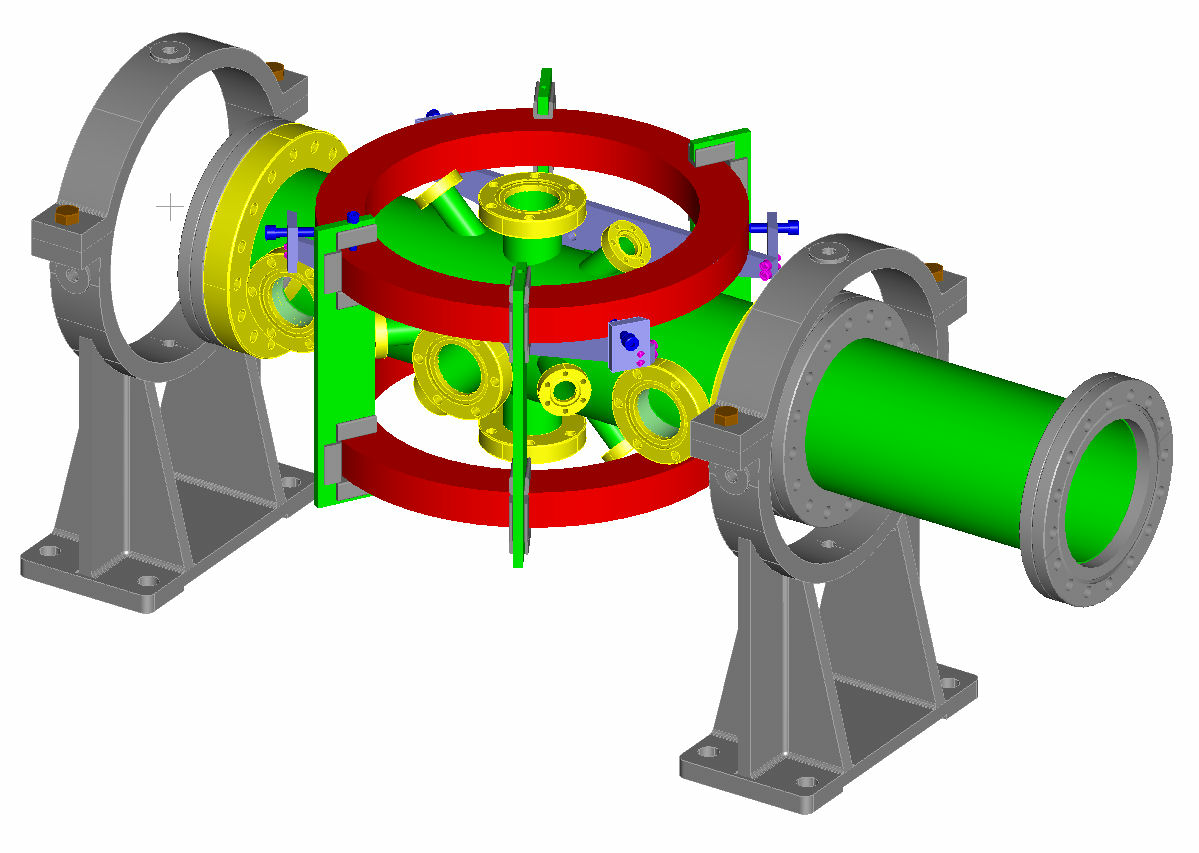
\includegraphics[scale=0.5]{figures/chamber.png} % TODO hacer que esto no quede horrible

    \caption[Esquema de la disposición de pines de la placa nRF51-DK de Nordic]{Esquema de la disposición de pines de la placa nRF51-DK de Nordic}

   \label{figuraNordicNRF51}
\end{figure}

La  carga de programas resulta sencilla, ya que solo debemos abrir un explorador de archivos de Windows. Confirmar que el nRF52 DK ha aparecido como una unidad extraíble llamado "JLINK". Esto permite programar el chip a bordo. Podremos cargar los programas a la placa arrastrando y soltando hacia la unidad.

\textbf{ARM Mbed} es una plataforma gratuita de prototipado rápido y experimentación con microcontroladores ARM. Provee a los desarrolladores una plataforma productiva para realizar pruebas conceptuales y prototipos en lenguaje de programación C/C++. Incluye amplia variedad de librerías, tutoriales y ejemplos, además de contar de una gran comunidad online de más de 130.000 desarrolladores de software, cuyos códigos son habitualmente accesibles a toda la comunidad.

Otro chip con procesador que nos pareció interesante fue el modelo CY8CKIT-042-BLE de la empresa Cypress que soporta 2 dispositivos: PSoC 4 BLE y  PRoC BLE.

El modelo escogido es el PSoC 4 BLE que provee de una completa solución para conectividad Bluetooth Low Energy. También monta una procesador ARM Cortex-M0 con una memoria flash de 128kB / 256kB y RAM de 16kB / 32kB. Dispone de 4 TCPWM1, 2 SCBs2, LCD4, I2S5, and 36 GPIOs.

\begin{figure}[h]%t=top, b=bottom, h=here
	\centering
    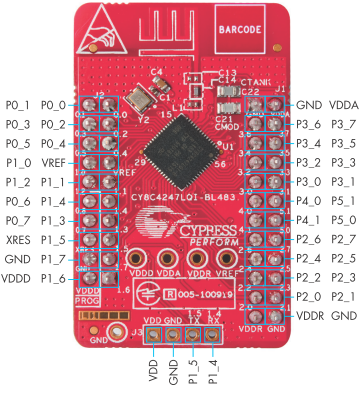
\includegraphics[width=\linewidth]{figures/cypress_psoc.PNG} % TODO hacer que esto no quede horrible

    \caption[TODO]{TODO}

   \label{figuraCypressPeque}
\end{figure}

\begin{figure}[h]%t=top, b=bottom, h=here
	\centering
    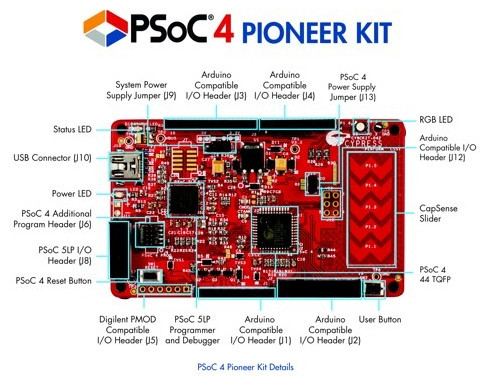
\includegraphics[scale=0.5]{figures/cypress_placa_desarrollo} % TODO hacer que esto no quede horrible

    \caption[TODO]{TODO}

   \label{figuraCypressGrande}
\end{figure}

El kit incluye una memoria extraible que conecta la placa por Bluetooth llamado Dongle USB CySmart (BLE Dongle) que se empareja con la herramienta de emulación principal CySmart. El emparejamiento con un entorno Windows hace que sea un potente entorno de depuración de Bluetooth LE.

\begin{figure}[h]%t=top, b=bottom, h=here
	\centering
    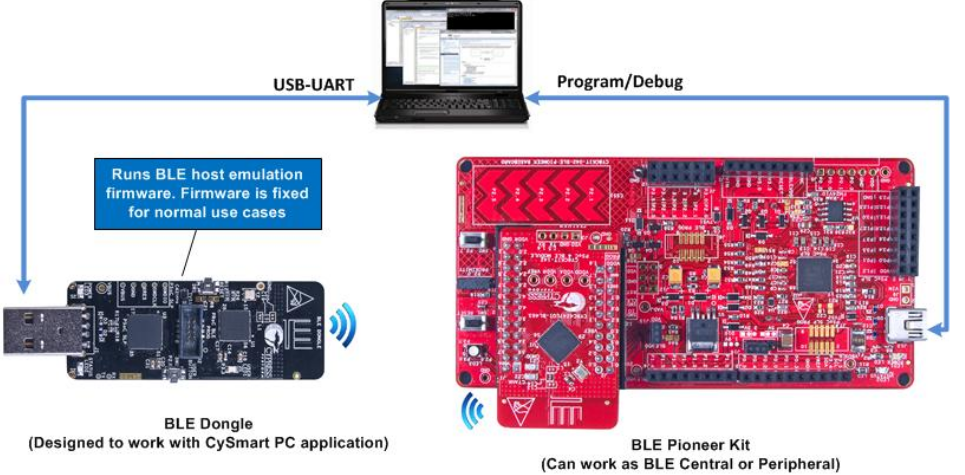
\includegraphics[scale=0.5]{figures/cypress_dongle.png} % TODO hacer que esto no quede horrible

    \caption[TODO]{TODO}

   \label{figuraCypressDongle}
\end{figure}

Este kit de desarrollo de Cypress es compatible con diseños a nivel de sistema mediante PSoC Creator, un software de desarrollo que contiene numerosos proyectos de ejemplo para proporcionar diseños integrados de señal mixta Bluetooth de baja energía, el lenguaje utilizado es C.

Es sencilla diseñar pues con arrastrar y soltar los componentes se añaden al panel principal obteniendo máxima flexibilidad de diseño.

\section{Conclusión}
\label{makereference3.5}

Tanto la placa nRF51-DK de Nordic como CY8CKIT-042-BLE de Cypress son dos placas de desarrollo perfectas para iniciar un proyecto con conectividad Bluetooth, las dos tienen idénticas características, conectores y periféricos, se les puede incluir una pila de botón CR2032 para darles autonomía y les respalda un software para desarrollo de las mismas.

En este punto tuvimos cierta controversia, ya que el software de Mbed de Nordic nos da la posibilidad de compilar código C++ en cualquier PC con internet gracias a su versión web. Nos ofrece una gran comunidad que es de agradecer y mucho contenido de ejemplos y tutoriales en la web oficial. Por contra no tiene modo depuración por pasos y eso dificulta su seguimiento y depuración. 

Por otro lado, PSoC Creator de Cypress nos ofrece un completo programa de escritorio muy visual al diseñar circuitos y un sistema “drag and drop” muy intuitivo. Permite modo depuración facilitando su programación. Por contra nos hemos encontrado con ciertas dudas que han sido difíciles de resolver en foros debido al poco contenido sobre el tema.